% -*- coding: utf-8; -*-
% vim: set fileencoding=utf-8 :
\documentclass[english,submission]{programming}
%% First parameter: the language is 'english'.
%% Second parameter: use 'submission' for initial submission, remove it for camera-ready (see 5.1)

\usepackage[backend=biber]{biblatex}
\addbibresource{example.bib}


%
% Packages and Commands specific to article (see 3)
%
% These ones  are used in the guide, replace with your own.
% 
\usepackage{multicol}
\lstdefinelanguage[programming]{TeX}[AlLaTeX]{TeX}{%
  deletetexcs={title,author,bibliography},%
  deletekeywords={tabular},
  morekeywords={abstract},%
  moretexcs={chapter},%
  moretexcs=[2]{title,author,subtitle,keywords,maketitle,titlerunning,authorinfo,affiliation,authorrunning,paperdetails,acks,email},
  moretexcs=[3]{addbibresource,printbibliography,bibliography},%
}%
\lstset{%
  language={[programming]TeX},%
  keywordstyle=\firamedium,
  stringstyle=\color{RosyBrown},%
  texcsstyle=*{\color{Purple}\mdseries},%
  texcsstyle=*[2]{\color{Blue1}},%
  texcsstyle=*[3]{\color{ForestGreen}},%
  commentstyle={\color{FireBrick}},%
}

\newcommand*{\CTAN}[1]{\href{http://ctan.org/tex-archive/#1}{\nolinkurl{CTAN:#1}}}
%%


%%%%%%%%%%%%%%%%%%
%% These data MUST be filled for your submission. (see 5.3)
\paperdetails{
  %% perspective options are: art, sciencetheoretical, scienceempirical, engineering.
  %% Choose exactly the one that best describes this work. (see 2.1)
  perspective=art,
  %% State one or more areas, separated by a comma. (see 2.2)
  %% Please see list of areas in http://programming-journal.org/cfp/
  %% The list is open-ended, so use other areas if yours is/are not listed.
  area={Social Coding, General-purpose programming},
  %% You may choose the license for your paper (see 3.)
  %% License options include: cc-by (default), cc-by-nc
  % license=cc-by,
}
%%%%%%%%%%%%%%%%%%

%%%%%%%%%%%%%%%%%%
%% These data are provided by the editors. May be left out on submission.
%\paperdetails{
%  submitted=2016-08-10,
%  published=2016-10-11,
%  year=2016,
%  volume=1,
%  issue=1,
%  articlenumber=1,
%}
%%%%%%%%%%%%%%%%%%
\definecolor{codegray}{gray}{0.9}
\newcommand{\code}[1]{\colorbox{codegray}{\texttt{#1}}}

\begin{document}

\title{Live probes for free}
%\subtitle{Preparing Articles for Programming}% optional
%\titlerunning{Preparing Articles for Programming} %optional, in case that the title is too long; the running title should fit into the top page column

\author[a]{Tobias Pape}
\authorinfo{is the author of this {LaTeX} class. Contact him at
  \email{tobias.pape@hpi.uni-potsdam.de}.}
\affiliation[a]{Hasso Plattner Institute, University of Potsdam, Germany}
\author{Cristina V. Lopes}
\authorinfo{is associate editor for the first two issues of The Art, Science,
  and Engineering of Programming. Contact her at \email{lopes@ics.uci.edu}.}
\affiliation{University of California, Irvine, USA}
\author[a]{Robert Hirschfeld}
\authorinfo{is chair of the AOSA steering committee. The Art, Science,
  and Engineering of Programming is published by AOSA. Contact Robert at \email{hirschfeld@hpi.uni-potsdam.de}.}

% \authorrunning{T. Pape, C. Lopes, R. Hirschfeld} % Optional, for long author lists

\keywords{programming journal, paper formatting, submission preparation} % please provide 1--5 keywords


%%%%%%%%%%%%%%%%%%%%%%%%%%%%%
% Please go to https://dl.acm.org/ccs/ccs.cfm and generate your Classification
% System [view CCS TeX Code] stanz and copy _all of it_ to this place.
%% From HERE
\begin{CCSXML}
<ccs2012>
<concept>
<concept_id>10002944.10011122.10003459</concept_id>
<concept_desc>General and reference~Computing standards, RFCs and guidelines</concept_desc>
<concept_significance>300</concept_significance>
</concept>
<concept>
<concept_id>10010405.10010476.10010477</concept_id>
<concept_desc>Applied computing~Publishing</concept_desc>
<concept_significance>300</concept_significance>
</concept>
</ccs2012>
\end{CCSXML}

\ccsdesc[300]{General and reference~Computing standards, RFCs and guidelines}
\ccsdesc[500]{Applied computing~Publishing}

% To HERE
%%%%%%%%%%%%%%%%%%%%%%%

\maketitle

% Please always include the abstract.
% The abstract MUST be written according to the directives stated in 
% http://programming-journal.org/submission/
% Failure to adhere to the abstract directives may result in the paper
% being returned to the authors.
\begin{abstract}
  %What is the broad context of the work? What is the importance of the general research area?
  \emph{Context}
  In his presentation "Inventing on Principles", Bret Victor demonstrates a live code editor: by specifying input values for a function, we can observe in real time the values taken by the variables during execution, as the code is written. 
  This information is often obtained using a language designed for live programming or by instrumentation of a specific runtime.
  % What problem or question does the paper address? How has this problem or question been addressed by others (if at all)?
  \emph{Inquiry}
  \dots
  % What was done that unveiled new knowledge?
  \emph{Approach}
  In this paper we propose to exploit the capabilities of debuggers to obtain the data needed to design a live code editor.
  % What new facts were uncovered? If the research was not results oriented, what new capabilities are enabled by the work?
  \emph{Knowledge}
  \dots
  % What argument, feasibility proof, artifacts, or results and evaluation support this work?
  \emph{Grounding}
  \dots
  % Why does this work matter?
  \emph{Importance}
  \dots
 
\end{abstract}
\section{Introduction}
\label{sec:introduction}

\section{Problem Overview}
\label{sec:problem-overview}

\section{Using the Debugger ?}
\label{sec:stack-recording}

\subsection{Stack Recording}

\begin{figure}[h]
  \centering
  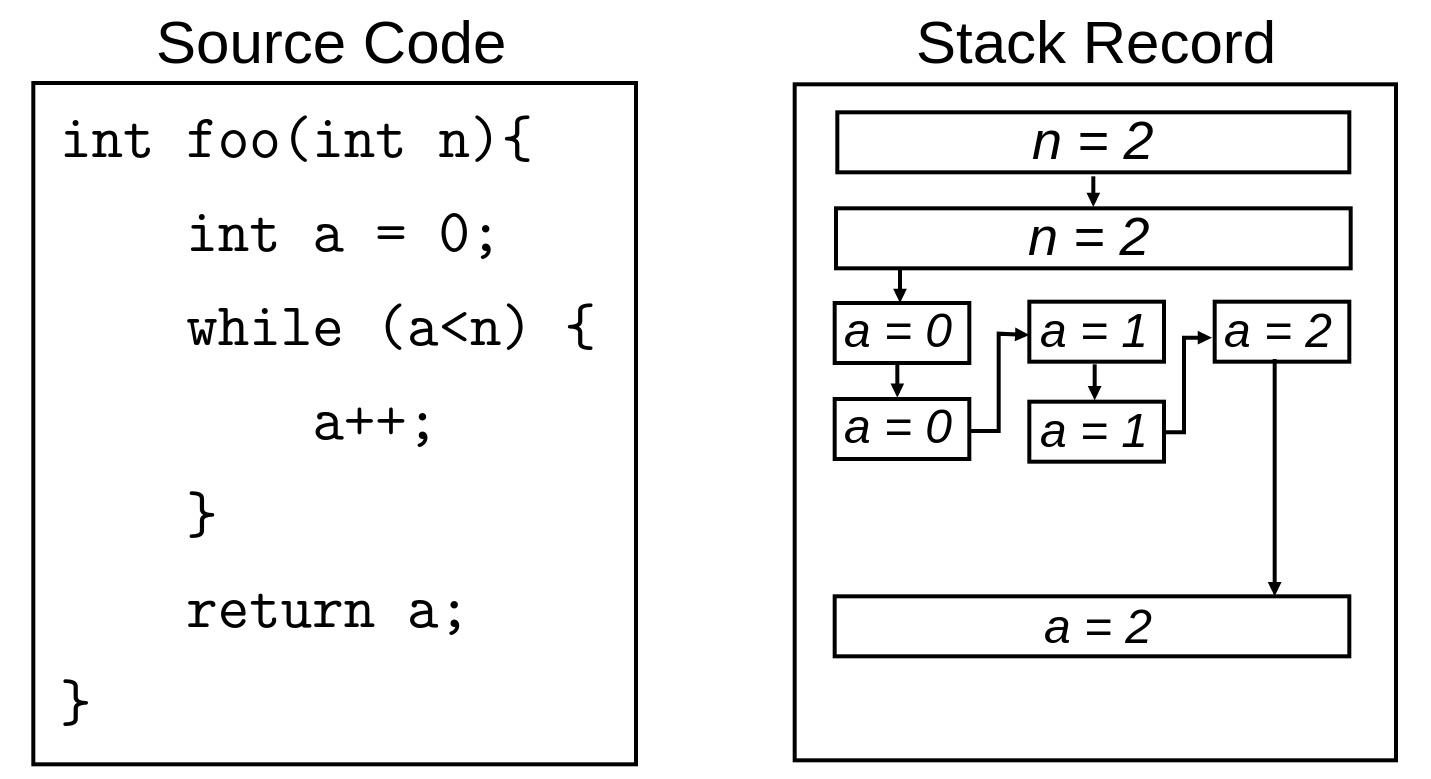
\includegraphics[width=0.8\linewidth]{img/stackrecord.png}
  \caption{Stack Recording example}
  \label{fig:stack-recording}
\end{figure}

In order to generate the data needed to probe a variable, we need to be able to retrieve the state of the variable during execution. 
This information is contained in the stackframe at the time of execution. 
However, we need to add spatial and temporal information to this: we need to associate each stackframe with the location in the code at which it was retrieved, and we also need to know the order in which these stackframes were retrieved.

In this paper, we introduce a structure for representing this data: a \textit{stack recording} \ref*{fig:stack-recording}. 
A stack trace represents the different stackframes in the form of a chain, where each stackframe has a reference to the corresponding line of source code. 
This representation allows us to maintain a link between the spatial location (the reference to the source code) and the temporal location (the order of these stackframes) of the execution.
This representation has several advantages: it is easy to construct from debugger information, and it applies to most programming languages.

\subsection{Keep Alive Agent}

\begin{figure}[h]
  \centering
  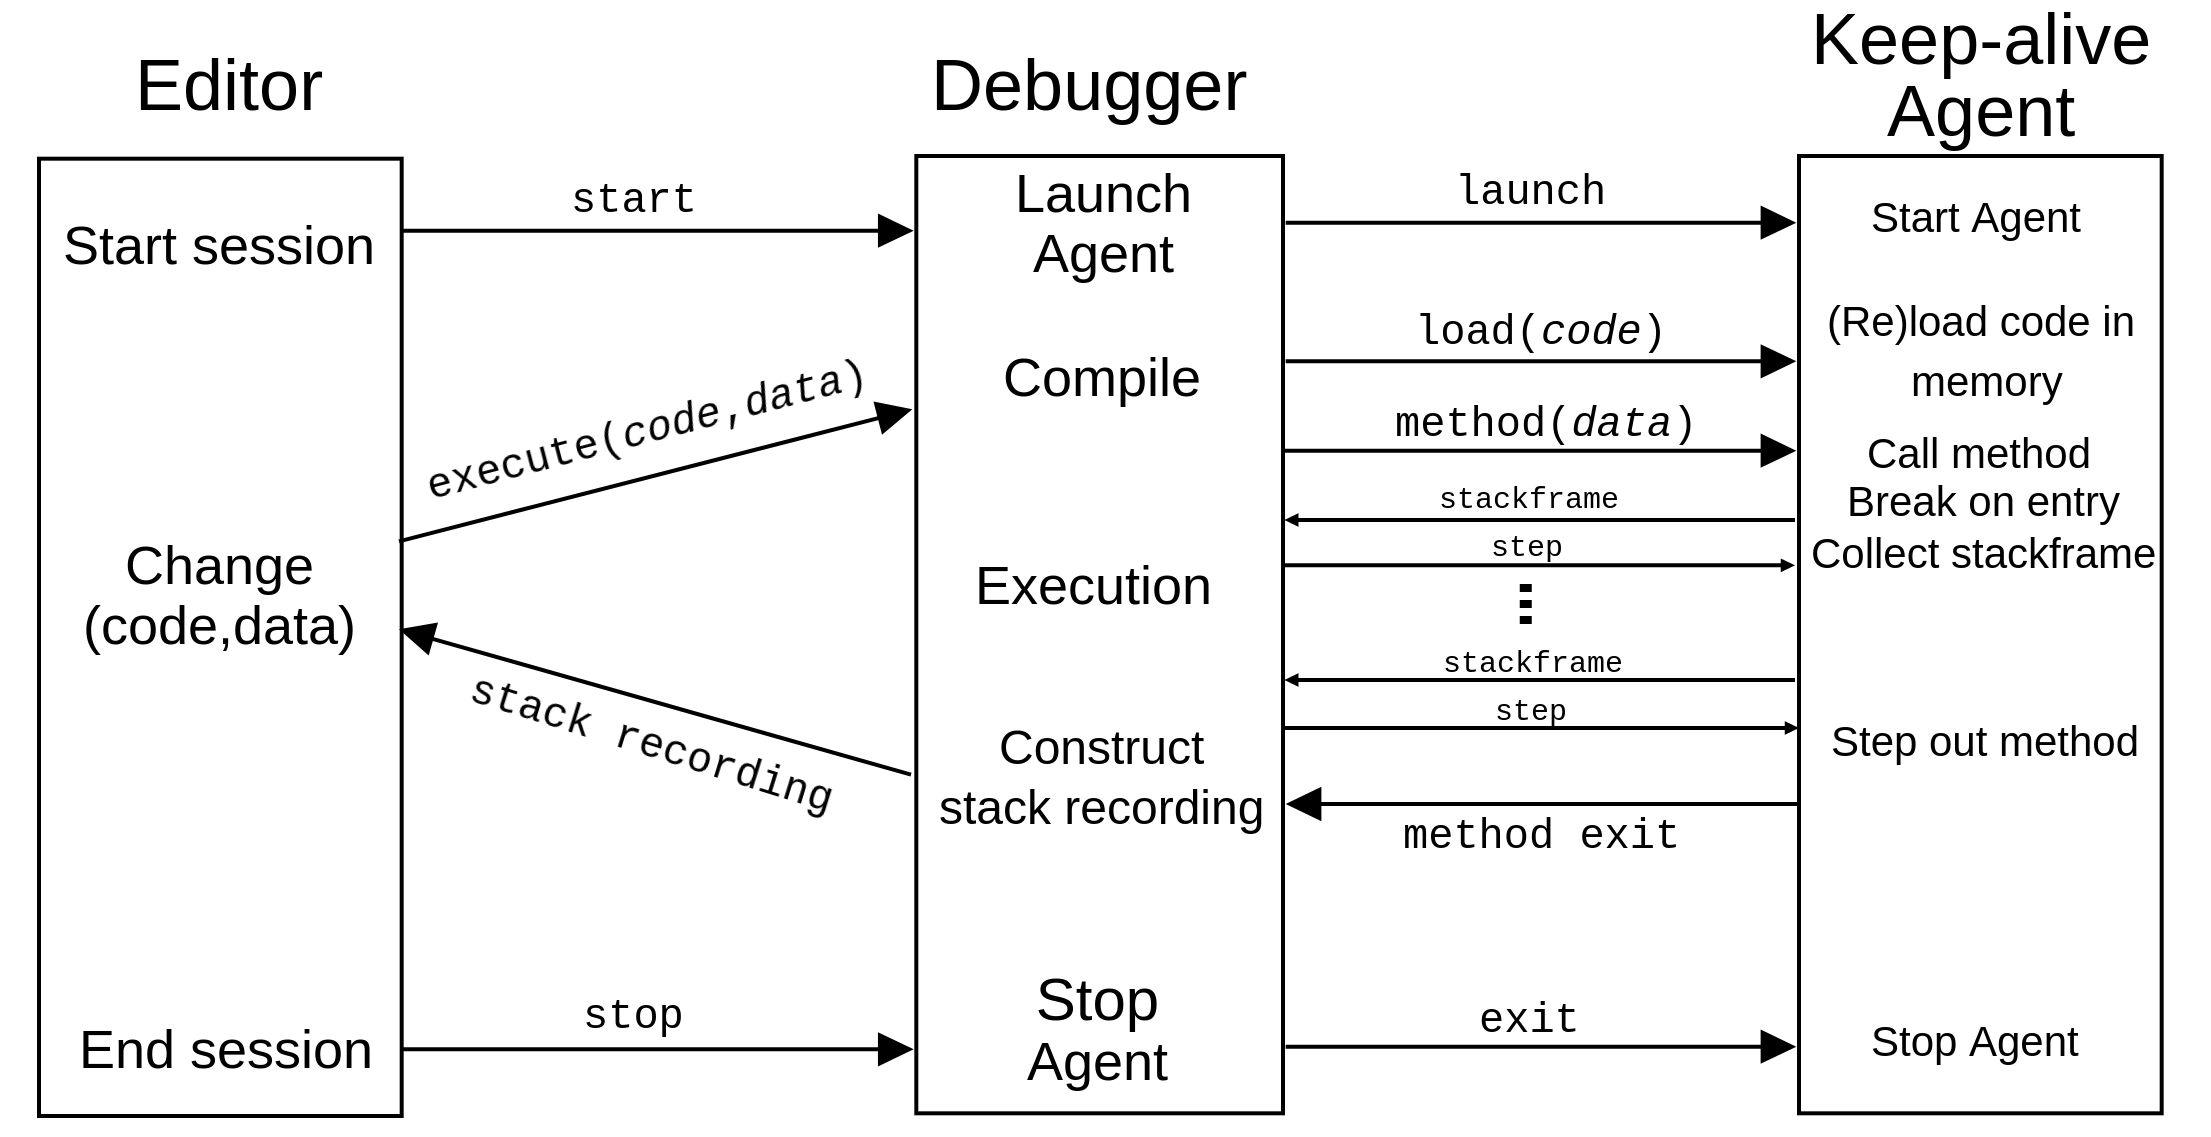
\includegraphics[width=0.8\linewidth]{img/keepalive_agent.png}
  \caption{Keep Alive Agent}
  \label{fig:keepalive-agent}
\end{figure}

A live environment must be able to react to two different events: a change in the code or a change in the test/input data. 
If the code changes, we need to re-execute the code, and in the case of a compiled language, we need to compile the new code first. 
If the data changes, we need to be able to re-execute the programme with the new data. 
In addition, it is necessary to keep compilation and execution times low enough to maintain an interactive experience with the user.

To meet these constraints, we propose to use the debugger on an intermediate program, a \textit{keep-alive agent}. 
This program keeps the debugger alive between executions and code changes to reduce initialisation times. 
The general operation of a keep-alive agent is shown in Figure \ref*{fig:keepalive-agent} :
\begin{itemize}
  \item At the start of the session, the debugger is started on the agent. Once initialised, the agent is paused.
  \item The target code is loaded into the agent and a breakpoint is set at the input of the target method.
  \item Execution of the target method triggers the breakpoint at the input of the method, and execution continues step by step to build the \textit{stack recording}.
\end{itemize}

\section{Live Probes in Java with JDI}
\label{sec:live-probes-java}

We initially developed a Java backend using JDI, a debugging interface for Java, to implement the concepts discussed in the previous section. The keep-alive agent includes a method for loading classes into the JVM.

When executing the target method, the arguments are created in the client JVM and then passed to the debugger JVM using the \code{mirrorOf} and \code{newInstance} methods from the reflection API. The target method is invoked using \code{invokeMethod}. 
To handle events from the JDI when breakpoints are set, a dedicated thread is used to prevent deadlocks.

If modifications are needed in the code of the target method, we employ the \code{redefineClasses} method. 
This method allows changing the content of a class loaded in the JVM using an array of byte codes. 
However, it has a limitation: it only works if the class signature remains unchanged. 
If the class structure is modified, restarting the debugger is necessary.

\section{Generalizing Live Probes with Debugger Adapter Protocol}
\label{sec:generalizing-live-probes}
The Debug Adapter Protocol (DAP), developed by Microsoft, is a standard method of communicating with a programming language debugger. It is compatible with various editors, including VS Code, and provides a unified interface for all programming languages. 

By exploiting this protocol, we have created a new language parametric backend, which we have implemented for the C, Python and Java programming languages. These languages are chosen to cover both compiled and interpreted languages. This backend offers an interface common to all three languages, which includes methods for starting and initialising the debugging server, loading and reloading code in the debugger, and executing a method while performing stack recording. 

These methods allow us to carry out stack recording independently of the chosen language and facilitate the future implementation of live programming interfaces. 

However, it is essential to develop a keep-alive agent specific to each language and to adapt these different methods to the debugging server. These methods depend on both the implementation of the debugging server and the keep-alive agent. Initialization in the DAP protocol is left to the discretion of the debugging server developer, which means that the initialization parameters must be configured for each language.

How the code is loaded also depends on the language. For interpreted languages such as Python, this presents no problem because the code can be interpreted while the agent is running. For Java, classpaths and classes can be added at runtime by redefining the JVM's ClassLoader in the keep-alive agent. For the C language, shared libraries are used to import new code and can be loaded from the agent.

Finally, execution for Java and Python is similar. Unlike the backend, which uses JDI, calling methods directly from the debugger does not trigger breakpoints. To remedy this, execution must be initiated from the agent and not by a debugger command. To this end, the Python and Java agents have fields for referencing a method and its arguments; when this information is entered, the agent launches execution.

\section{Evaluation}
\label{sec:evaluation}
\subsection{Demo : A Small C Live Programming Environment}
\label{sec:demo-small-c}
\subsection{Performance}
\label{sec:performance}
\section{Related Work}
\label{sec:related-work}

Example-Based Live Programming for Everyone\cite{10.1145/3426428.3426919} : Use GraalVM/Truffle to get live information from the code of multiple languages.

Example Centric Programming\cite{10.1145/1052883.1052894} : Use BeanShell(custom JVM) to get live information. Prototype for Java in Eclipse.

Usable Live Programming\cite{10.1145/2509578.2509585} : New language for live programming(Ying Yang) with incremental compilation. Live programming environment for this language.
Use source location to relate execution and code(=> almost like stack recording that link stackframe and code location)

Scalable Omniscient Debugging\cite{10.1145/1297105.1297067} : Omniscient debugging with a lot of data. Use a lot of memory to store all the data.
In this paper they record almost everything, we only record the stackframe.

\section{Conclusion}
\label{sec:conclusion}

\printbibliography

\end{document}

% Local Variables:
% TeX-engine: luatex
% End:
